% Standalone tikz figure illustrating axonal pub/sub tree healing
% via routed re-subscribe.  Shows BOTH a leaf subscriber and a
% sub-axon (with its own subtree) re-attaching to a live branch
% after their parent dies — so healing repairs not just individual
% subscribers but whole subtrees.
%
% Build:  tectonic Axonal-PubSub-Healing.tex
% Convert: pdftoppm -png -r 200 Axonal-PubSub-Healing.pdf out

\documentclass[tikz,border=8pt]{standalone}
\usepackage{tikz}
\usetikzlibrary{positioning, arrows.meta, shapes.geometric, fit, backgrounds}
\usepackage{xcolor}
\definecolor{rust}{RGB}{185,78,54}
\definecolor{rustsoft}{RGB}{212,168,150}
\definecolor{inkmuted}{RGB}{102,102,102}

\begin{document}
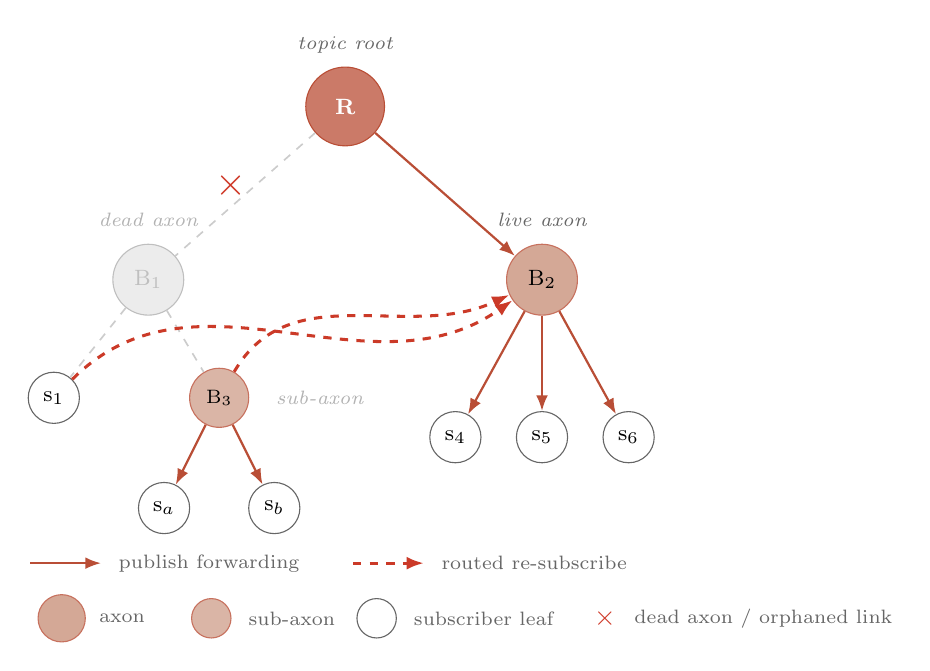
\begin{tikzpicture}[font=\small,
    root/.style={circle, draw=rust, fill=rust!75!white, text=white,
                 font=\footnotesize\bfseries, minimum size=10mm, inner sep=0pt},
    branch/.style={circle, draw=rust!80, fill=rustsoft,
                   font=\footnotesize, minimum size=9mm, inner sep=0pt},
    subaxon/.style={circle, draw=rust!80, fill=rustsoft!85,
                    font=\scriptsize, minimum size=7.5mm, inner sep=0pt},
    deadbranch/.style={circle, draw=gray!50, fill=gray!15,
                       font=\footnotesize, minimum size=9mm, inner sep=0pt,
                       text=gray!50},
    leaf/.style={circle, draw=inkmuted, fill=white,
                 font=\footnotesize, minimum size=6.5mm, inner sep=0pt},
    pubarr/.style={-{Latex[length=2mm]}, thick, color=rust},
    subarr/.style={-{Latex[length=2.2mm]}, dashed, color=rust!75!red, line width=1.1pt},
    deadedge/.style={gray!40, line width=0.6pt, dashed},
]

% ─── Root + two branches ──────────────────────────────────────────
\node[root] (R) at (4, 5.2) {R};
\node[font=\scriptsize\itshape, color=inkmuted, anchor=south] at (4, 5.75) {topic root};

\node[deadbranch] (B1) at (1.5, 3) {B$_1$};
\node[font=\scriptsize\itshape, color=gray!60, anchor=south] at (1.5, 3.55) {dead axon};

\node[branch] (B2) at (6.5, 3) {B$_2$};
\node[font=\scriptsize\itshape, color=inkmuted, anchor=south] at (6.5, 3.55) {live axon};

% ─── Under B1: one leaf and one sub-axon ──────────────────────────
% s1 is a direct leaf; B3 is a sub-axon (intermediate role) with its
% own leaf children.  When B1 dies, BOTH s1 and B3 must re-subscribe;
% B3 carries its s_a, s_b subtree intact across the move.
\node[leaf]    (s1) at (0.3, 1.5) {s$_1$};
\node[subaxon] (B3) at (2.4, 1.5) {B$_3$};
\node[font=\scriptsize\itshape, color=gray!60, anchor=west] at (3.0, 1.5) {sub-axon};

% B3's own children — these stay attached to B3 through the re-stitching
\node[leaf] (sa) at (1.7, 0.1) {s$_a$};
\node[leaf] (sb) at (3.1, 0.1) {s$_b$};

% ─── Under B2: three leaves (still publish-connected) ──────────────
\node[leaf] (s4) at (5.4, 1) {s$_4$};
\node[leaf] (s5) at (6.5, 1) {s$_5$};
\node[leaf] (s6) at (7.6, 1) {s$_6$};

% ─── Edges ───────────────────────────────────────────────────────
% R → B1: broken
\draw[deadedge] (R) -- (B1);
\node[color=rust!70!red, font=\Large\bfseries] at (2.55, 4.2) {$\times$};

% R → B2: intact publish
\draw[pubarr] (R) -- (B2);

% B1 → s1 (orphaned leaf) and B1 → B3 (orphaned sub-axon)
\draw[deadedge] (B1) -- (s1);
\draw[deadedge] (B1) -- (B3);

% B3 → its own children — STILL ALIVE, B3 keeps serving s_a, s_b
% even while it itself is re-subscribing.  Solid publish-forward.
\draw[pubarr] (B3) -- (sa);
\draw[pubarr] (B3) -- (sb);

% B2 → leaves: publish forwarding
\draw[pubarr] (B2) -- (s4);
\draw[pubarr] (B2) -- (s5);
\draw[pubarr] (B2) -- (s6);

% ─── Routed re-subscribes: only s1 and B3 need to issue them ──────
% B3's subtree (s_a, s_b) does NOT individually re-subscribe — the
% whole subtree moves with B3 to its new parent.  This is what
% "tree healing" actually looks like at scale: a single subscribe
% per surviving subtree, not one per leaf.
\draw[subarr] (s1) to[out=45, in=215] (B2);
\draw[subarr] (B3) to[out=60, in=205] (B2);

% No in-flight annotation overlaying the diagram — the legend
% explains the edge types and the figure caption (in the explainer)
% will carry the subtree-preservation point in prose.

% ─── Legend ──────────────────────────────────────────────────────
% Two rows.  Top row: edge styles.  Bottom row: node styles + dead.
\begin{scope}[shift={(0, -0.6)}]
  % Edge legend
  \draw[pubarr] (0.0, 0) -- (0.9, 0);
  \node[font=\scriptsize, color=inkmuted, anchor=west] at (1.0, 0) {publish forwarding};

  \draw[subarr] (4.1, 0) -- (5.0, 0);
  \node[font=\scriptsize, color=inkmuted, anchor=west] at (5.1, 0) {routed re-subscribe};

  % Node + dead legend
  \node[branch, minimum size=6mm] at (0.4, -0.7) {};
  \node[font=\scriptsize, color=inkmuted, anchor=west] at (0.75, -0.7) {axon};

  \node[subaxon, minimum size=5mm] at (2.3, -0.7) {};
  \node[font=\scriptsize, color=inkmuted, anchor=west] at (2.65, -0.7) {sub-axon};

  \node[leaf, minimum size=5mm] at (4.4, -0.7) {};
  \node[font=\scriptsize, color=inkmuted, anchor=west] at (4.75, -0.7) {subscriber leaf};

  \node[color=rust!70!red, font=\normalsize\bfseries] at (7.3, -0.7) {$\times$};
  \node[font=\scriptsize, color=inkmuted, anchor=west] at (7.55, -0.7) {dead axon / orphaned link};
\end{scope}

\end{tikzpicture}
\end{document}
